\documentclass[tikz,border=4pt,11pt]{standalone}
\usepackage{amsmath}
\usetikzlibrary{arrows.meta}
\definecolor{ink}{RGB}{42,52,64}
\definecolor{first}{RGB}{146,79,26}
\definecolor{second}{RGB}{26,99,111}

% Beraha--Kahane--Weiss limit set of the zeros of P_n(x)=1+x^n+(x+1)^n:
% the arc |x|=1 with |x+1|<=1, the arc |x+1|=1 with |x|<=1, and the parts
% of the line Re x=-1/2 with |Im x|>=sqrt(3)/2, meeting at (-1+-i sqrt3)/2.
% The dots are the 30 zeros of P_30 (computed to high precision, rounded to
% three decimals); the two zeros -1/2 +- 9.541i lie outside the window.
% Grey labels name the dominant term(s) in each region.

\begin{document}
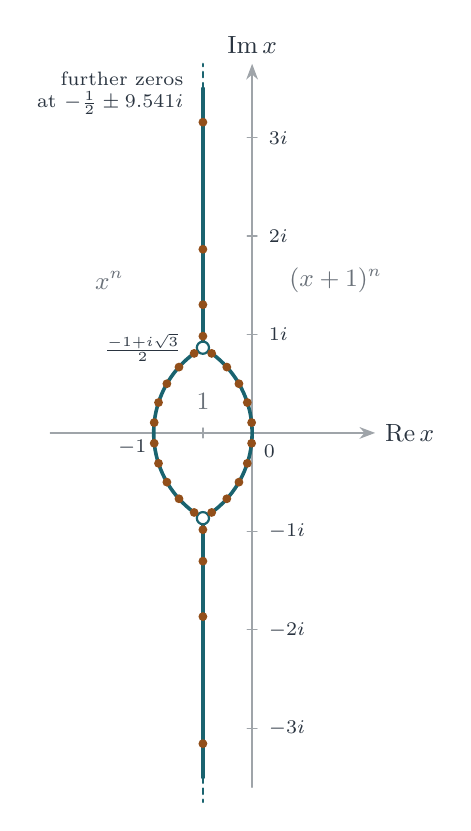
\begin{tikzpicture}[x=1.25cm,y=1.25cm,text=ink,line cap=round,line join=round]
  % axes
  \draw[ink!45,line width=.5pt,-{Stealth[length=2mm]}] (-2.05,0) -- (1.25,0)
    node[right,font=\small,text=ink] {$\operatorname{Re}x$};
  \draw[ink!45,line width=.5pt,-{Stealth[length=2mm]}] (0,-3.6) -- (0,3.75)
    node[above,font=\small,text=ink] {$\operatorname{Im}x$};
  \foreach \x in {-1,-0.5} {
    \draw[ink!45,line width=.5pt] (\x,-.05) -- (\x,.05);
  }
  \node[font=\scriptsize,anchor=north east,inner sep=1pt] at (-1.04,-.04) {$-1$};
  \foreach \y in {-3,-2,-1,1,2,3} {
    \draw[ink!45,line width=.5pt] (-.05,\y) -- (.05,\y);
    \node[font=\scriptsize,anchor=west] at (.07,\y) {$\y i$};
  }
  \node[font=\scriptsize,anchor=north west] at (.02,-.02) {$0$};

  % limit set
  \begin{scope}[second,line width=1.3pt]
    \draw (120:1) arc[start angle=120,end angle=240,radius=1];
    \draw (-1,0) ++(-60:1) arc[start angle=-60,end angle=60,radius=1];
    \draw (-0.5,0.866) -- (-0.5,3.5);
    \draw (-0.5,-0.866) -- (-0.5,-3.5);
    \draw[line width=.8pt,dash pattern=on 2pt off 2pt] (-0.5,3.5) -- (-0.5,3.75);
    \draw[line width=.8pt,dash pattern=on 2pt off 2pt] (-0.5,-3.5) -- (-0.5,-3.75);
  \end{scope}
  \foreach \s in {1,-1}
    \draw[second,fill=white,line width=.8pt] (-0.5,\s*0.866) circle (2.2pt);

  % zeros of P_30
  \foreach \p in {
    (-0.995,-0.105),(-0.995,0.105),(-0.951,-0.309),(-0.951,0.309),
    (-0.866,-0.500),(-0.866,0.500),(-0.743,-0.669),(-0.743,0.669),
    (-0.589,-0.808),(-0.589,0.808),(-0.500,-3.157),(-0.500,-1.866),
    (-0.500,-1.303),(-0.500,-0.983),(-0.500,0.983),(-0.500,1.303),
    (-0.500,1.866),(-0.500,3.157),(-0.411,-0.808),(-0.411,0.808),
    (-0.257,-0.669),(-0.257,0.669),(-0.134,-0.500),(-0.134,0.500),
    (-0.049,-0.309),(-0.049,0.309),(-0.005,-0.105),(-0.005,0.105)}
    \fill[first] \p circle (1.6pt);

  % dominant terms
  \node[ink!70,font=\small] at (-1.45,1.55) {$x^n$};
  \node[ink!70,font=\small] at (0.85,1.55) {$(x+1)^n$};
  \node[ink!70,font=\small] at (-0.5,.32) {$1$};

  % annotations
  \node[font=\scriptsize,anchor=east,align=right] at (-0.6,3.45) {further zeros\\at $-\tfrac12\pm 9.541i$};
  \node[font=\scriptsize,anchor=east] at (-0.62,0.866) {$\tfrac{-1+i\sqrt3}{2}$};
\end{tikzpicture}
\end{document}
